\chapter{Results}

\section{Hyper-Parameter Optimization}

    In order to significantly reduce the cost of evaluation (re-training
    the whole model from scratch with a different set of hyper-parameters),
    the training set used for hyper-parameter tuning has been
    limited to the PSICOV150 families.
    Hyperopt stopped after only 32 iterations with a maximum of 48,9 \%
    of best-L PPV on the 30 validation proteins.

    \begin{figure}[H]
        \begin{center}
            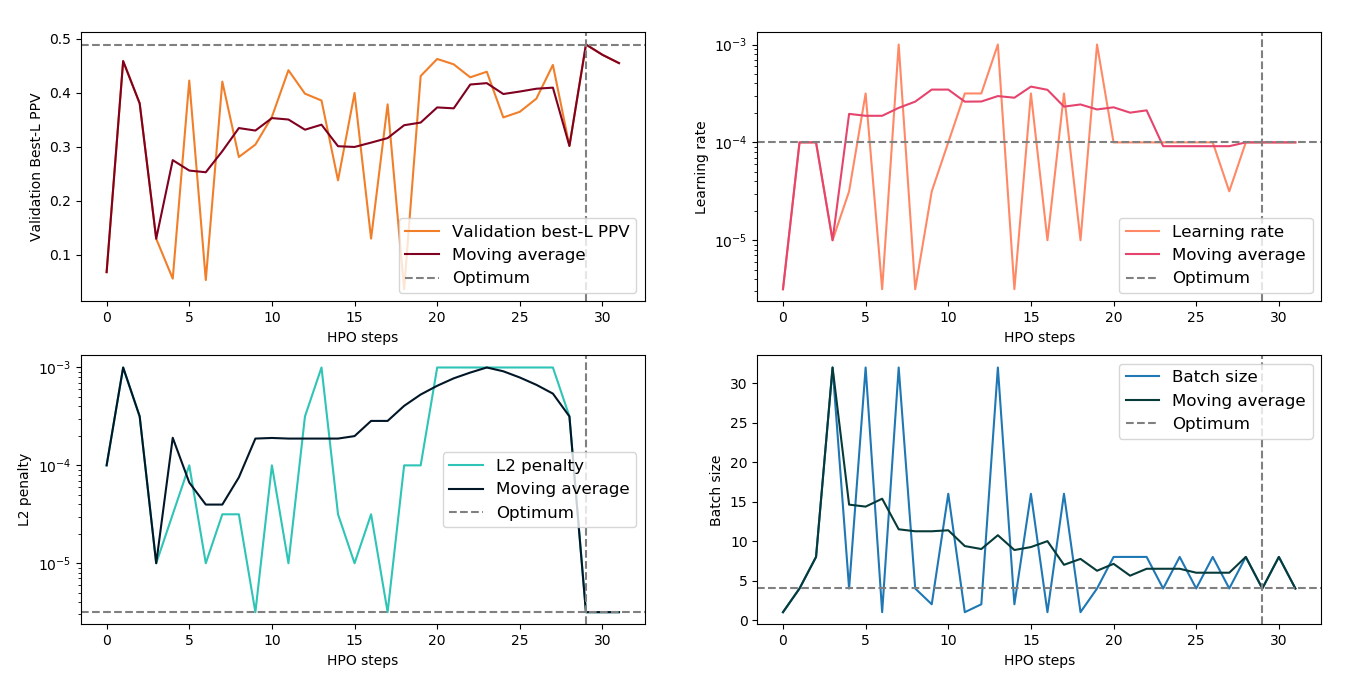
\includegraphics[width=\textwidth, keepaspectratio]{imgs/hpo.png}
            \caption{Performance and hyper-parameter values as a function of the number
            of Hyper-Parameter Optimization (HPO) iterations.
            Top left figure illustrates the optimal point whose value on x-axis
            is given by the HPO iteration that yields highest validation Best-L PPV.
            Optimal values for the learning rate, L2 penalty and batch size are denoted
            by dashed lines in top right, bottom left and bottom right figures, respectively.}
            \label{hpoparams}
        \end{center}
    \end{figure}

    As can be observed in top left figure in \ref{hpoparams}, a high-quality solution (local maximum)
    was found in the very first iterations, but the algorithm continued to explore and
    found its best solution after 30 iterations with a completely different set of parameters:
    L2 regularization parameter changed from $10^{-3}$ to $\frac{1}{2} 10^-{5}$ and
    batch size changed from $32$ proteins to only $4$. Because these two solutions
    are very distant in the hyper-parameter space and have similar performance,
    it can be suggested that the latter is the search space is multimodal.

    \begin{figure}[H]
        \begin{center}
            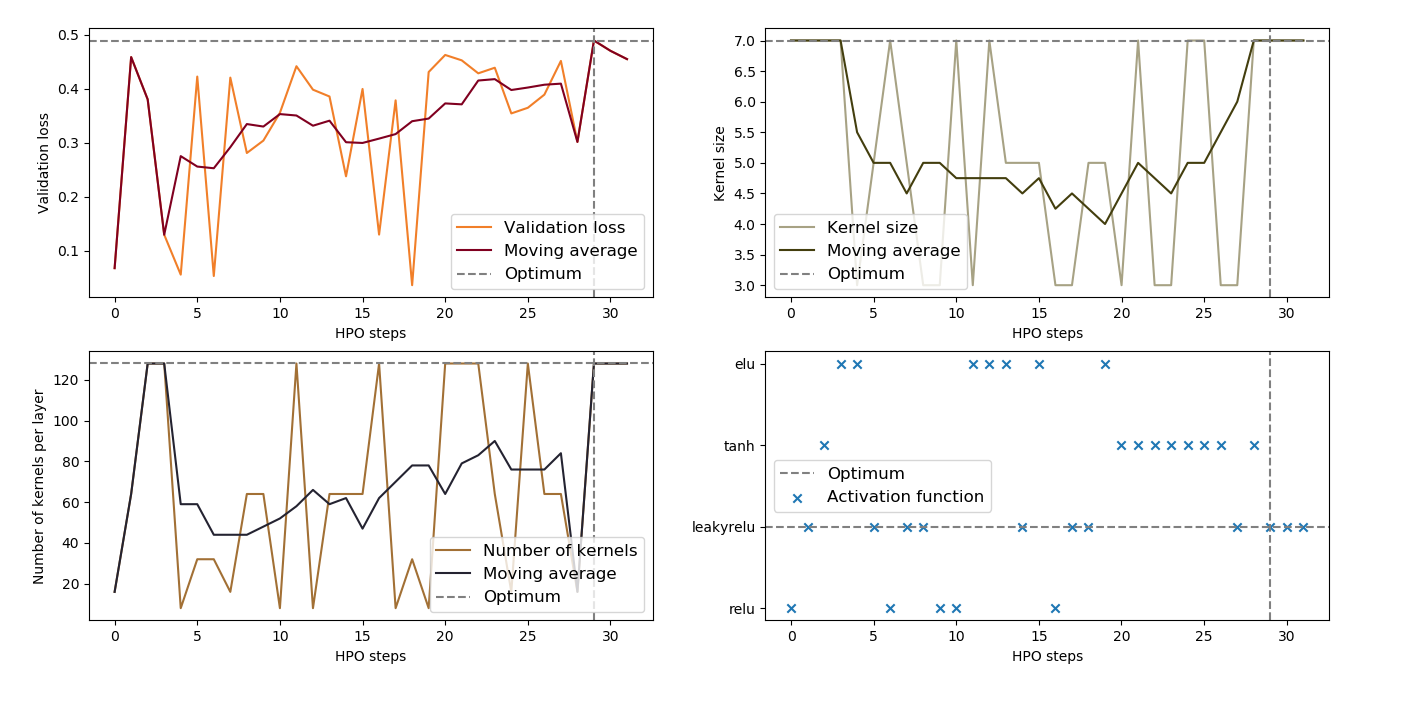
\includegraphics[width=\textwidth, keepaspectratio]{imgs/hpo2.png}
            \caption{Performance and hyper-parameter values as a function of the number
            of Hyper-Parameter Optimization (HPO) iterations.
            Top left figure illustrates the optimal point whose value on x-axis
            is given by the HPO iteration that yields highest validation Best-L PPV.
            Optimal values for kernel size, number of kernels and activation function are denoted
            by dashed lines in top right, bottom left and bottom right figures, respectively.}
            \label{hpoparams2}
        \end{center}
    \end{figure}

    Optimal hyper-parameter values are provided in table \ref{besthp}.
    It turned out that batch normalization is required, which is consistent
    with the fact that a very large network depth has been found
    (3 + 18 + 18 layers). A batch size of 4 is sufficient, which makes sense
    since each example is a protein of size $L$ containing potentially
    $L (L - 1) / 2$ residue pairs and each residue pair is a statistical
    example \textit{per se}.

    \begin{table}[H]
        \centering
        \begin{tabular}{lll}
          \hline
          Module & Hyper-parameter & Set of values \\
          \hline
          \hline
          General & Batch size & $4$ \\
                  & Batch normalization & $\top$ \\
                  & Track running state & $\bot$ \\
                  & Learning rate & $10^{-4}$ \\
                  & L2 penalty & $10^{-4}$ \\
                  & Parameter optimization & $\text{Adam}$ \\
                  & Activation function & $\text{LeakyReLU}$ \\
                  & Use global modules & $\top$ \\
          \hline
          Global module & Depth & $3$ \\
          \hline
          1-dimensional module & Depth & $18$ \\
                               & Filter size & $7$ \\
                               & Number of filters & $128$ \\
          \hline
          2-dimensional module & Depth & $18$ \\
                               & Filter size & $7$ \\
                               & Number of filters & $128$ \\
          \hline
        \end{tabular}
        \captionof{table}{Set of hyper-parameter values obtained at optimal point.}
        \label{besthp}
    \end{table}

    A L2 regularization parameter of $10^{-4}$ has been found.
    However, this value has been replaced
    by $10^{-5}$ for training the final model on the whole training set since
    the latter contains much more proteins than PSICOV150 alone, alleviating
    the need for regularization.

    \begin{figure}[H]
        \begin{center}
            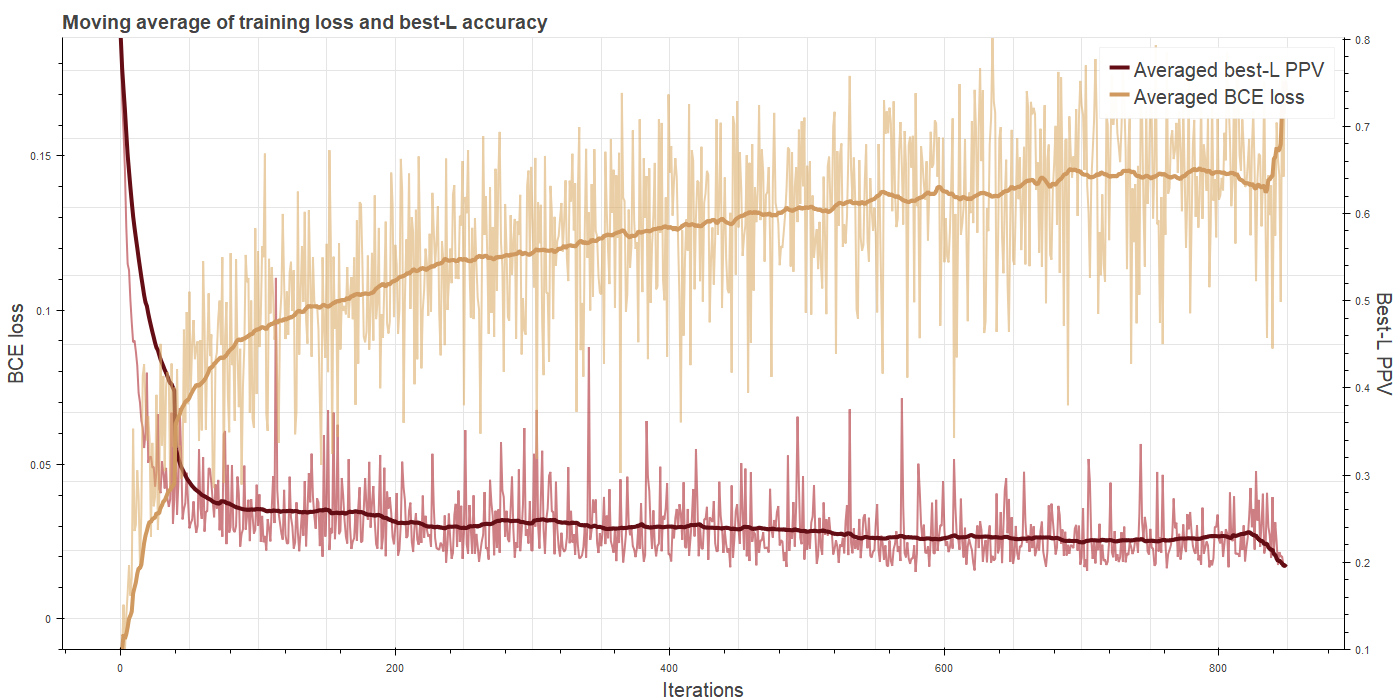
\includegraphics[width=\textwidth, keepaspectratio]{imgs/loss.png}
            \caption{Binary Cross-Entropy loss and best-L PPV computed on
              a rolling window of batches, related to the training phase of the model
              with best hyper-parameters.}
            \label{lossandppv}
        \end{center}
    \end{figure}

    Convergence of the final model on PSICOV150 is shown in figure~\ref{lossandppv}.
    It can be noticed that binary cross-entropy is directly and inversely
    related to the training PPV. The neural network takes approximately 850
    batches to converge. However, when trained on the whole training set, it takes
    approximately 16 000 batches and 4 days before the algorithm converges.

\section{Model evaluation on the different benchmark sets}

    Performance measured in table~\ref{benchmark} is the PPV obtained
    by only considering the top $L$ predicted probabilities as predicted
    contacts (see section \ref{evaluationmetrics} for more details about the evaluation
    metrics). In this way, the evaluation is based only on the contacts
    the predictive model is the most confident about.
    As can be observed, best-L PPV is significantly lower for short range contacts,
    regardless of the method used. Indeed, the number of residue pairs having a
    sequence separation between 6 \AA{} and 12 \AA{} is much smaller then for a
    separation between 12 \AA{} and 24 \AA{} (medium range) or above 24 \AA{} (long range).
    Furthermore, proteins with few or no short range native contacts will obviously yield
    a lot of false positives.
    Short range best-L PPV is thus computed on the basis of much less confident
    predictions than in the other cases, making the evaluation much more disadvantageous.
    This phenomenon is only due to the metric itself and does not appropriately reflect how hard
    the prediction task is: predicting short range contacts is actually easier to do
    than predicting long range ones.

    \subsection{CASP11 targets}

    \begin{table}[H]
        \centering
        \resizebox{\textwidth}{!}{
        \begin{tabular}{|l|ccc|ccc|ccc|}
            \hline
            & & CASP11 & & & CAMEO & & & Membrane & \\
            \hline
            Method & Short & Medium & Long & Short & Medium & Long & Short & Medium & Long \\
            \hline
            \hline
            Proposed method & 0.26 & 0.30 & 0.39 & 0.22 & 0.26 & 0.28 & 0.14 & 0.18 & 0.32 \\
            RaptorX-Contact & 0.28 & 0.35 & 0.55 & 0.23 & 0.28 & 0.42 & 0.16 & 0.22 & 0.47 \\
            PconsC3         & 0.25 & 0.29 & 0.40 & 0.21 & 0.23 & 0.27 & 0.15 & 0.19 & 0.33 \\
            MetaPSICOV & 0.26 & 0.31 & 0.39 & 0.22 & 0.22 & 0.28 & 0.16 & 0.21 & 0.35 \\
            PlmDCA & 0.14 & 0.16 & 0.27 & 0.11 & 0.13 & 0.19 & 0.08 & 0.11 & 0.21 \\
            PSICOV & 0.14 & 0.15 & 0.24 & 0.13 & 0.14 & 0.18 & 0.09 & 0.11 & 0.20 \\
            mfDCA & 0.13 & 0.15 & 0.22 & 0.10 & 0.11 & 0.15 & 0.09 & 0.12 & 0.24 \\
            \hline
        \end{tabular}
        }
        \captionof{table}{Best-L PPV of different methods on short,
        medium and long-range contacts. Results are shown for the three
        different benchmark sets: CASP11 targets, CAMEO proteins, and
        the benchmark set of membrane proteins.}
        \label{benchmark}
    \end{table}

    Unsupervised methods (namely DCA and PSICOV) are clearly outperformed on a very large margin
    by other methods. Proposed model seems to perform similarly to PConsC3, while being still significantly far
    from the state-of-the-art RaptorX-Contact, regardless of the evaluation metric.
    Tables \ref{casp11benchmark}, \ref{cameobenchmark} and \ref{membranebenchmark} show the overall
    performance on the three different test sets individually.

    \subsection{CAMEO targets}

    \begin{table}[H]
        \centering
        \resizebox{\textwidth}{!}{
        \begin{tabular}{|l|cccc|cccc|cccc|}
            \hline
            Method & \multicolumn{4}{|c|}{Short range} & \multicolumn{4}{|c|}{Medium range} & \multicolumn{4}{|c|}{Long range} \\
            \hline
            & L/10 & L/5 & L/2 & L & L/10 & L/5 & L/2 & L & L/10 & L/5 & L/2 & L \\
            \hline
            \hline
            EVfold          & 0.25 & 0.21 & 0.15 & 0.12 & 0.33 & 0.27 & 0.19 & 0.13 & 0.37 & 0.33 & 0.25 & 0.19 \\
            PSICOV          & 0.29 & 0.23 & 0.15 & 0.12 & 0.34 & 0.27 & 0.18 & 0.13 & 0.38 & 0.33 & 0.25 & 0.19 \\
            plmDCA          & 0.35 & 0.28 & 0.17 & 0.12 & 0.40 & 0.32 & 0.21 & 0.14 & 0.43 & 0.39 & 0.31 & 0.23 \\
            Gremlin         & 0.32 & 0.26 & 0.17 & 0.12 & 0.39 & 0.31 & 0.21 & 0.14 & 0.42 & 0.38 & 0.30 & 0.23 \\
            CCMpred         & 0.35 & 0.27 & 0.17 & 0.12 & 0.40 & 0.31 & 0.21 & 0.14 & 0.44 & 0.40 & 0.31 & 0.23 \\
            MetaPSICOV      & 0.69 & 0.58 & 0.39 & 0.25 & 0.69 & 0.59 & 0.42 & 0.28 & 0.60 & 0.54 & 0.45 & 0.35 \\
            RaptorX-Contact & 0.82 & 0.70 & 0.46 & 0.28 & 0.85 & 0.76 & 0.55 & 0.35 & 0.81 & 0.77 & 0.68 & 0.55 \\
            Proposed method & 0.68 & 0.57 & 0.40 & 0.26 & 0.71 & 0.61 & 0.44 & 0.32 & 0.69 & 0.62 & 0.50 & 0.39 \\
            \hline
        \end{tabular}
        }
        \captionof{table}{Best-L/k PPV of different methods on the CASP11 targets with different values for L.}
        \label{casp11benchmark}
    \end{table}

    PlmDCA, Gremlin and CCMpred perform similarly, which is consistent with the fact that they all three rely on
    pseudo-likelihood direct coupling analysis. Proposed method outperforms METAPSICOV mostly on medium-range and long-range
    contacts on the CASP11 targets, with a 4 \% increase of the best-L long-range PPV.

    \subsection{Membrane proteins}

    \begin{table}[H]
        \centering
        \resizebox{\textwidth}{!}{
        \begin{tabular}{|l|cccc|cccc|cccc|}
            \hline
            Method & \multicolumn{4}{|c|}{Short range} & \multicolumn{4}{|c|}{Medium range} & \multicolumn{4}{|c|}{Long range} \\
            \hline
            & L/10 & L/5 & L/2 & L & L/10 & L/5 & L/2 & L & L/10 & L/5 & L/2 & L \\
            \hline
            \hline
            EVfold          & 0.17 & 0.13 & 0.11 & 0.09 & 0.23 & 0.19 & 0.13 & 0.10 & 0.25 & 0.22 & 0.17 & 0.13 \\
            PSICOV          & 0.20 & 0.15 & 0.11 & 0.08 & 0.24 & 0.19 & 0.13 & 0.09 & 0.25 & 0.23 & 0.18 & 0.13 \\
            plmDCA          & 0.22 & 0.16 & 0.11 & 0.09 & 0.27 & 0.22 & 0.14 & 0.10 & 0.30 & 0.26 & 0.20 & 0.15 \\
            Gremlin         & 0.23 & 0.18 & 0.12 & 0.09 & 0.27 & 0.22 & 0.14 & 0.10 & 0.30 & 0.26 & 0.20 & 0.15 \\
            CCMpred         & 0.21 & 0.17 & 0.11 & 0.08 & 0.27 & 0.22 & 0.14 & 0.10 & 0.31 & 0.26 & 0.20 & 0.15 \\
            MetaPSICOV      & 0.56 & 0.47 & 0.31 & 0.20 & 0.53 & 0.45 & 0.32 & 0.22 & 0.47 & 0.42 & 0.33 & 0.25 \\
            RaptorX-Contact & 0.67 & 0.57 & 0.37 & 0.23 & 0.69 & 0.61 & 0.42 & 0.28 & 0.69 & 0.65 & 0.55 & 0.42 \\
            Proposed method & 0.58 & 0.47 & 0.32 & 0.22 & 0.56 & 0.47 & 0.35 & 0.26 & 0.51 & 0.47 & 0.37 & 0.28 \\
            \hline
        \end{tabular}
        }
        \captionof{table}{Best-L/k PPV of different methods on the CAMEO targets with different values for L.}
        \label{cameobenchmark}
    \end{table}

    Proposed method outperforms METAPSICOV on the CAMEO targets, no matter whether predicted contacts are
    short, medium or long-range. Methods based on pseudo-likelihood DCA still perform similarly, while
    being more accurate than PSICOV.

    \begin{table}[H]
        \centering
        \resizebox{\textwidth}{!}{
        \begin{tabular}{|l|cccc|cccc|cccc|}
            \hline
            Method & \multicolumn{4}{|c|}{Short range} & \multicolumn{4}{|c|}{Medium range} & \multicolumn{4}{|c|}{Long range} \\
            \hline
            & L/10 & L/5 & L/2 & L & L/10 & L/5 & L/2 & L & L/10 & L/5 & L/2 & L \\
            \hline
            \hline
            EVfold          & 0.16 & 0.13 & 0.09 & 0.07 & 0.28 & 0.22 & 0.13 & 0.09 & 0.44 & 0.37 & 0.26 & 0.18 \\
            PSICOV          & 0.22 & 0.16 & 0.10 & 0.07 & 0.29 & 0.21 & 0.13 & 0.09 & 0.42 & 0.34 & 0.23 & 0.16 \\
            plmDCA          & 0.27 & 0.19 & 0.11 & 0.08 & 0.36 & 0.26 & 0.15 & 0.10 & 0.52 & 0.45 & 0.31 & 0.21 \\
            Gremlin         & 0.26 & 0.18 & 0.11 & 0.08 & 0.35 & 0.25 & 0.14 & 0.09 & 0.51 & 0.42 & 0.29 & 0.20 \\
            CCMpred         & 0.27 & 0.19 & 0.11 & 0.07 & 0.37 & 0.26 & 0.15 & 0.10 & 0.52 & 0.45 & 0.32 & 0.21 \\
            MetaPSICOV      & 0.45 & 0.35 & 0.22 & 0.14 & 0.49 & 0.40 & 0.27 & 0.18 & 0.61 & 0.55 & 0.42 & 0.30 \\
            RaptorX-Contact & 0.60 & 0.46 & 0.27 & 0.16 & 0.66 & 0.53 & 0.33 & 0.22 & 0.78 & 0.73 & 0.62 & 0.47 \\
            Proposed method & 0.38 & 0.30 & 0.21 & 0.14 & 0.45 & 0.37 & 0.26 & 0.18 & 0.58 & 0.52 & 0.41 & 0.32 \\
            \hline
        \end{tabular}
        }
        \captionof{table}{Best-L/k PPV of different methods on 398 membrane proteins with different values for L.}
        \label{membranebenchmark}
    \end{table}

    As can be observed in table \ref{membranebenchmark}, proposed model is comparatively less accurate when
    only top $L/10$ predictions are considered and gets comparatively better when $k$ decreases.
    As a consequence, it performs similarly to METAPSICOV when $L$ contacts are used.
    Overall, proposed model performs not as good as for the two previous datasets.

\section{Sensitivity to the number of sequence homologs}

    \subsection{CASP11 targets}

    Figure \ref{sensitivity} shows the comparative robustness
    of the method to the number of sequence homologs
    on CASP11 targets. On the basis of the regressions, it can be observed that
    the method is comparatively more accurate than plmDCA on proteins with
    fewer sequence homologs. The phenomenon is even more present with short-range contacts,
    where the method performance is almost invariant to the number of homologs.

    \begin{figure}[H]
        \begin{center}
            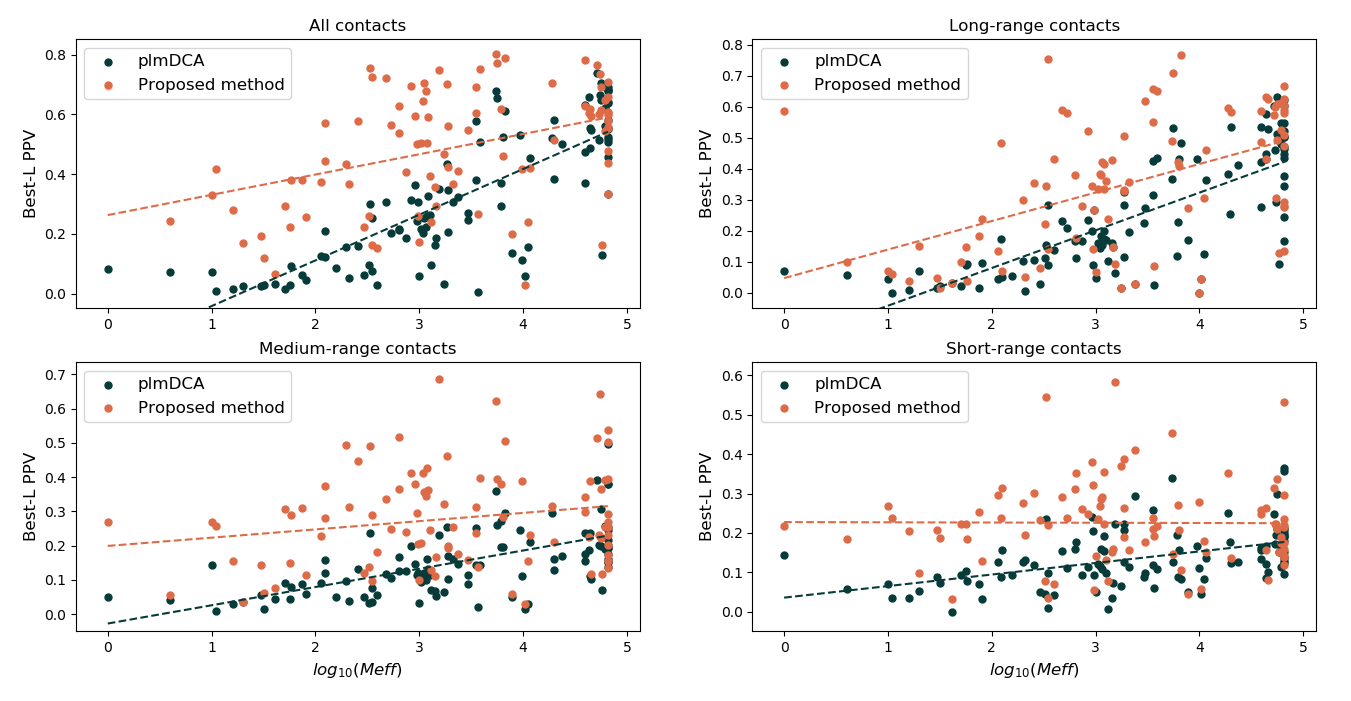
\includegraphics[width=\textwidth, keepaspectratio]{imgs/Meff.png}
            \caption{Performance as a function of the logarithm of the effective
            number of homologous sequences. Top figure shows the results on
            CASP11 targets for different types of contacts. Bottom left and bottom right figures
            focus on medium-range and long-range contacts, respectively.}
            \label{sensitivity}
        \end{center}
    \end{figure}

    \subsection{CAMEO targets}

    When evaluated on CAMEO targets, proposed model has a significantly better overall performance
    compared to plmDCA, but comparable dependence on the number of sequence homologs.
    However it can be observed as in the case of CASP11 targets that accuracy is more robust
    when computed on the basis of short-range contacts.

    \begin{figure}[H]
        \begin{center}
            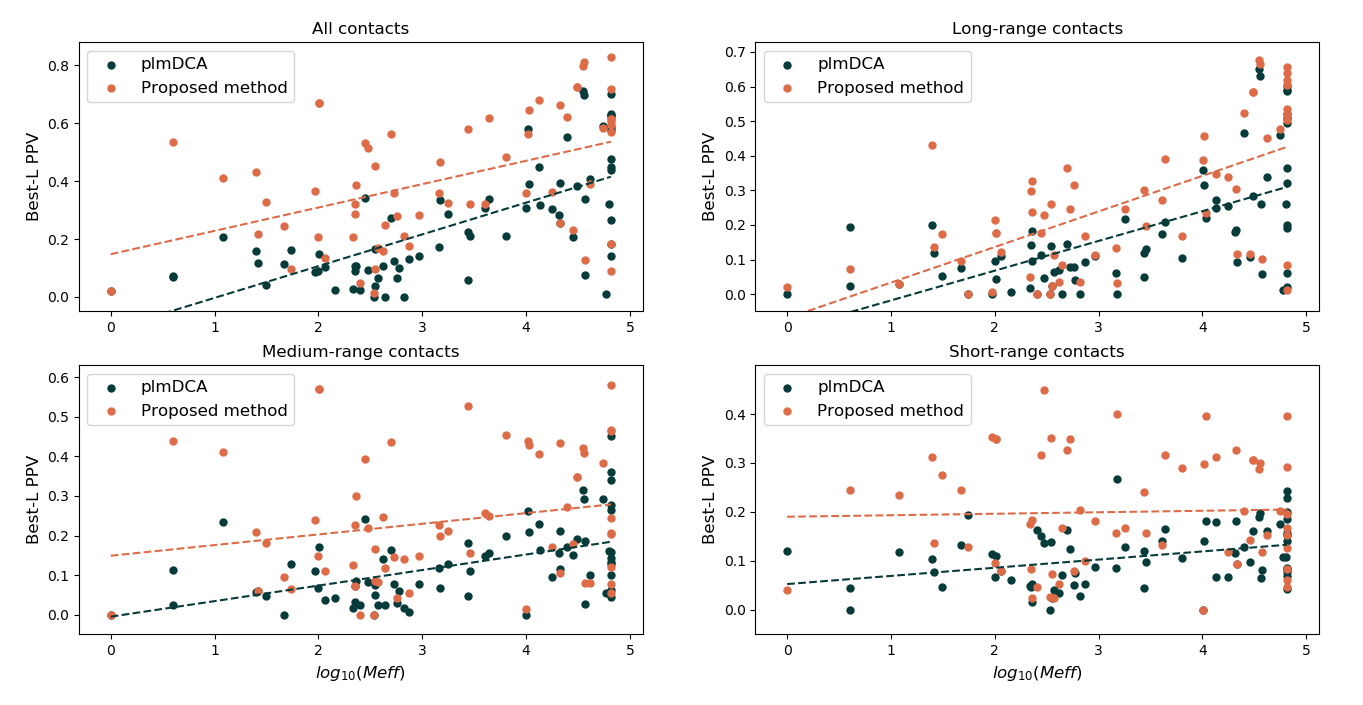
\includegraphics[width=\textwidth, keepaspectratio]{imgs/Meff_cameo.png}
            \caption{Performance as a function of the logarithm of the effective
            number of homologous sequences. Top figure shows the results on
            CAMEO targets for different types of contacts. Bottom left and bottom right figures
            focus on medium-range and long-range contacts, respectively.}
            \label{sensitivity_cameo}
        \end{center}
    \end{figure}

    \subsection{Membrane proteins}

    Figure \ref{sensitivity_membrane} confirms the observation made in the previous section:
    Performance gain introduced by the model w.r.t. DCA methods on membrane proteins is
    less important than on the two other datasets.

    \begin{figure}[H]
        \begin{center}
            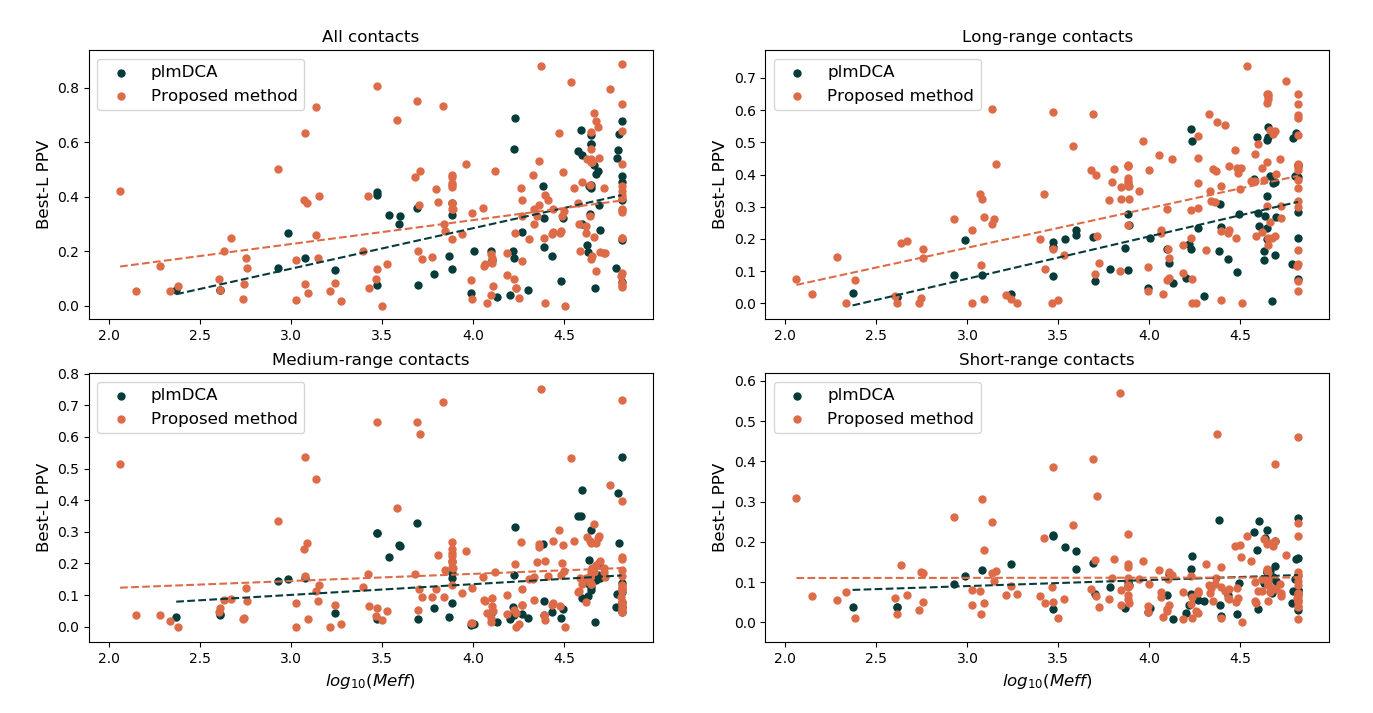
\includegraphics[width=\textwidth, keepaspectratio]{imgs/Meff_membrane.png}
            \caption{Performance as a function of the logarithm of the effective
            number of homologous sequences. Top figure shows the results on
            membrane proteins for different types of contacts. Bottom left and bottom right figures
            focus on medium-range and long-range contacts, respectively.}
            \label{sensitivity_membrane}
        \end{center}
    \end{figure}

\section{Further analysis on hard CAMEO targets}

    As can be observed in figure~\ref{analysis_4xrwa}, proposed method is able
    to refine GaussDCA predictions from a best-L PPV of 47,2 \% up to 83 \%
    for the di-domain ARO/CYC with PDB code 4XRWA~\cite{caldara2015structural}.
    A very large number of sequence homologs are available for this protein (65535),
    which partly explains the success in predicting long-range contacts.
    The two domains of the protein lay back-to-back with their
    beta sheets being anti-parallel.
    Antiparallel beta sheets are accurately predicted, but contacts between beta strands
    and helices do not seem to account in the top $L$ predictions.

    \begin{figure}[H]
        \begin{center}
            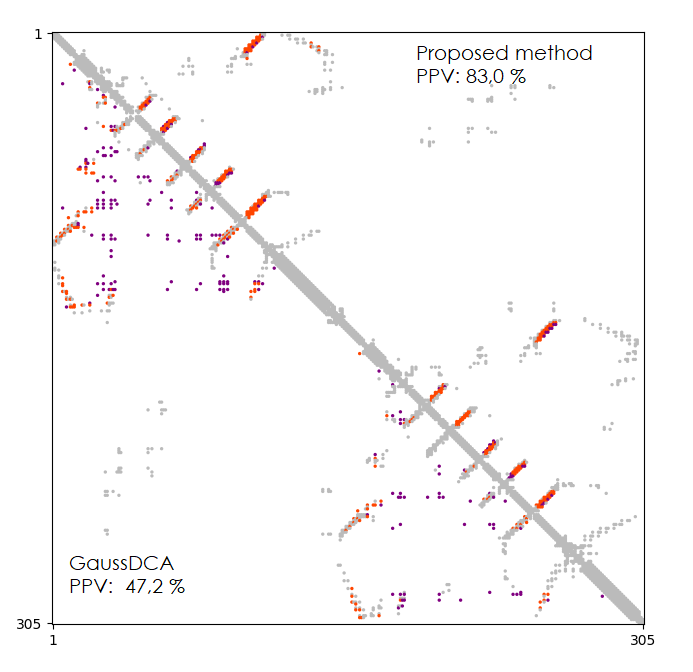
\includegraphics[width=\textwidth, keepaspectratio]{imgs/4XRWA.png}
            \caption{Comparison of the contact maps predicted for protein PDB:4XRWA
                by the proposed method and GaussDCA, respectively. True positives
                are highlighted in orange and false positives in purple.}
            \label{analysis_4xrwa}
        \end{center}
    \end{figure}

    It is noteworthy that the proposed model often completely fails at providing
    high-quality contact maps for proteins that are mainly alpha.
    Figure 5.8 shows predictions for the C-terminal domain of
    regnase-1~\cite{yokogawa2016structural}, composed of 3 $\alpha$-helices.
    False positives are mostly short-range predicted contacts, and the model fails at 
    finding any true contact between the first and the second helices.

    \begin{figure}[H]
        \begin{center}
            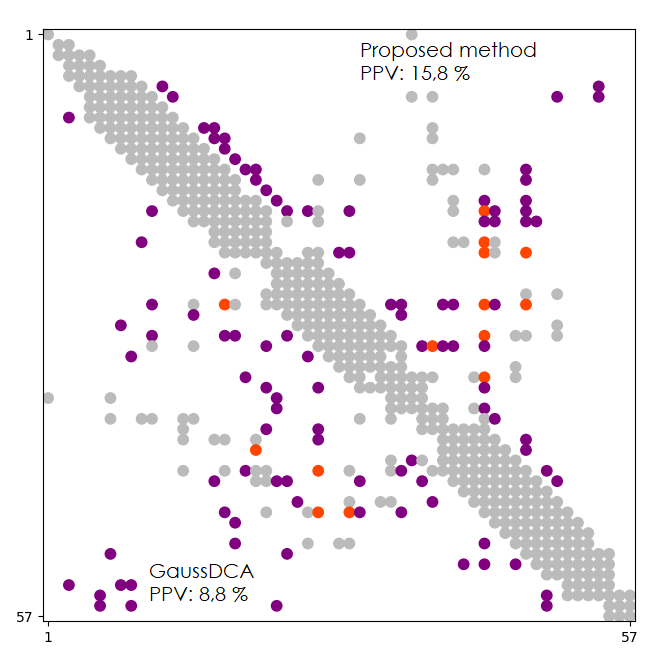
\includegraphics[width=\textwidth, keepaspectratio]{imgs/2N5LA.png}
            \caption{Comparison of the contact maps predicted for protein PDB:2N5LA
                by the proposed method and GaussDCA, respectively. True positives
                are highlighted in orange and false positives in purple.}
            \label{analysis_2N5LA}
        \end{center}
    \end{figure}

    Figure 5.9 is interesting as it shows predictions for a protein
    with 926 homologs but where most of them are much shorter. This has the effect
    to fill the multiple alignment matrix with gaps and yield poor
    evolutionary coupling predictions.
    Despite the ability of the model to improve contacts predicted by GaussDCA between the
    120 first residues of the sequence, it remains unable to accurately predict
    contacts on the second part of the sequence, highlighting the limits of the
    refinement abilities of deep architectures.

    \begin{figure}[H]
        \begin{center}
            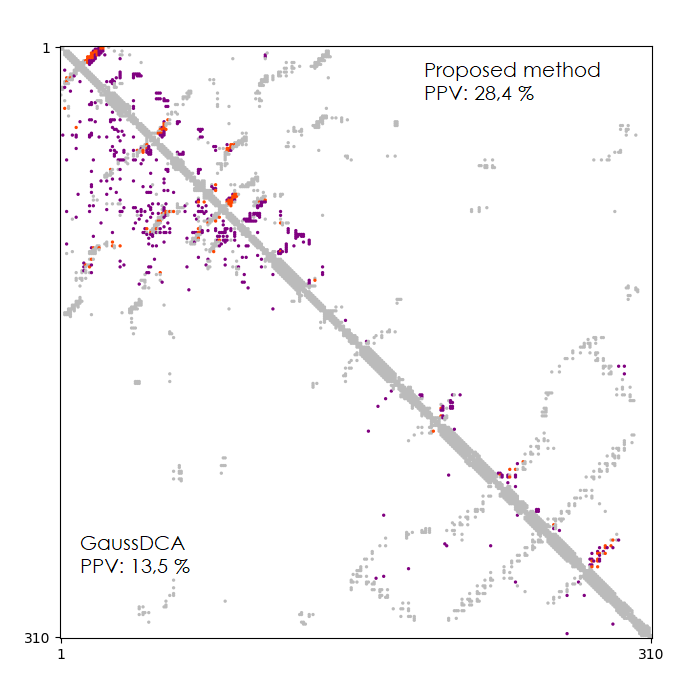
\includegraphics[width=\textwidth, keepaspectratio]{imgs/3X27D.png}
            \caption{Comparison of the contact maps predicted for protein PDB:3X27D
                by the proposed method and GaussDCA, respectively. True positives
                are highlighted in orange and false positives in purple.}
            \label{analysis_3X27D}
        \end{center}
    \end{figure}
